\section{Описание методов и инструментов для реализации}

\subsection{Система для промышленного интернета вещей}

Как было описано в предыдущим разделе 1,
промышленный анализ данных предоставляет идеи для создания
интеллектуальной системы для автоматизации и повышения
эффективности работы промышленных устройств.
Одной из множества компаний, которая ведет деятельность в данной области,
является компания Omnicube, которая, как уже говорилось,
имеет свою универсальную систему для множества
задач не только промышленного интернета вещей,
но интернета вещей в общем, то есть задачи,
решаемые данной системы, не ограничиваются промышленной отраслью.
Реализация решения для обнаружения и прогнозирования
неисправностей решается в контексте данной системы.
Опишем данную систему.

\begin{figure}[h]
    \center{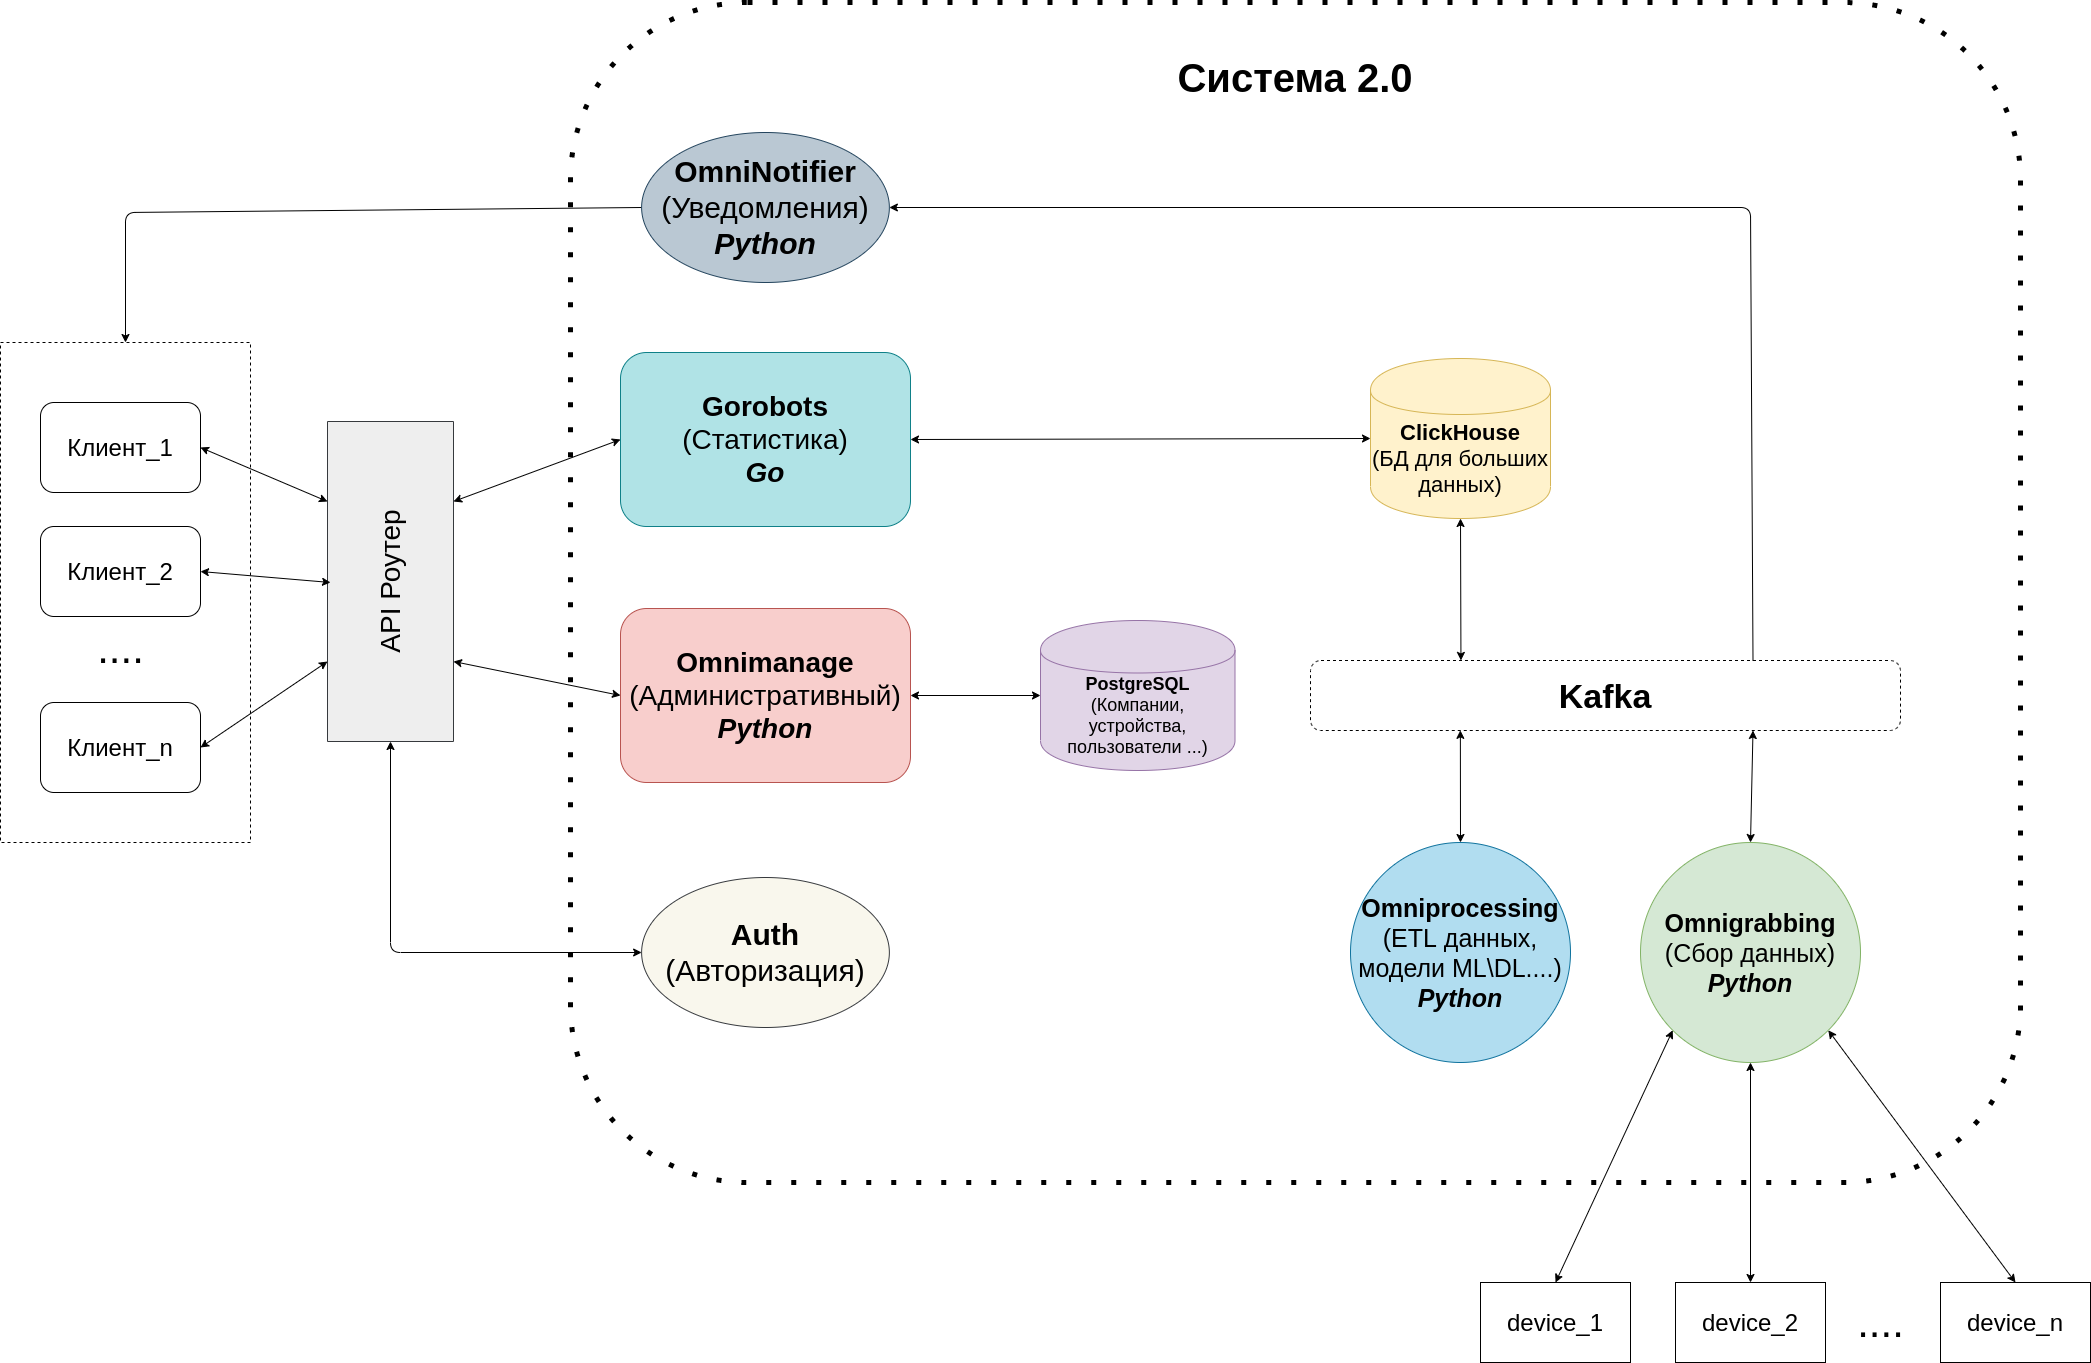
\includegraphics[width=15cm]{sys2.png}}
    \caption{Разработанная система для интернета вещей}
    \label{sys2}
\end{figure}

Система имеет микросервисную архитектуру (рисунок \ref{sys2}).
Микросервисная архитектура представляет собой рассмотрение
разрабатываемого приложения как совокупности связанных сервисов,
каждый их которых отвечает за какую-то часть общей системы,
а также решает свою определенную задачу.
Такой подход имеет свои преимущества и недостатки
Основным преимуществом является модульность,
которая позволяет разрабатывать и поддерживать
компоненты независимо друг от друга.
Недостатками являются:
высокая сложность разработки,
сложный процесс развертывания системы
на собственных кластерах,
и, особенно, на кластерах клиентов.

Основными взаимодействующими с системой структурами являются клиенты и устройства клиентов.
Каждое клиентское устройство соединяется с системой при помощи инженеров компании Omnicube
с учетом специфики самих устройств. Например, для станков лазерной резки Навигатор
использовались датчики, которые устанавливались на критически важные узлы, с которых собиралась необходимая информация.
Помимо этого, сами устройства клиентов иногда предоставляют функционал, который позволяет собирать данные без установки датчиков.
Далее, данные устройств агрегируются и обрабатываются также с учетом специфики устройств.
Обработанные данные выдаются клиентам в виде пользовательского интерфейса, примером которого является
интерфейс для предприятия Сеспель с данными станка лазерной резки Навигатор.

Главными узлами системы являются два микросервиса: omnimanage и gorobots.
Микросервис omnimanage отвечает за обработку первичных данных клиента:
сведения о клиенте, сведения о пользователях компании клиента,
сведения об устройствах клиента (но не сами данные устройств),
сведения о ролях пользователей для авторизации и т.д.
Gorobots отвечает за обработку собранной с устройств
статистики: вычисляет основные статистические показатели (среднее, дисперсию, КПД).
Omnimanage написан на языке Python с использованием базы данных PostgreSQL.
Gorobots написан на языке Go, данные в этом микросервисе берутся из базы данных ClickHouse.

Микросервис omnigrabbing отвечает за сбор и первоначальную обработку данных клиентских устройств.
в данном микросервисе происходит конвертация в необходимых формат для отправления данных в Kafka,
и последующую загрузку в ClickHouse.

Kafka -- платформа для обработки потоковых данных в реальном времени.
Проект направлен на создание унифицированной высокопроизводительной платформы 
с низкой задержкой для обработки потоков данных в реальном времени.
Kafka использует двоичный протокол на основе TCP,
а также системы для обработки асинхронных данных.
Такой брокер был выбран по причине большого количества поступающих данных.
Kafka позволяет гибко решать задачи обработки большого количества асинхронных данных \cite{kafka}.


ClickHouse - это быстрая система управления базами данных OLAP с открытым исходным кодом.
Данная система ориентирована на столбчатую структуру,
а также позволяет генерировать аналитические отчеты с использованием SQL-запросов в режиме реального времени.
База данных была выбрана по причине высокой нагрузки,
заключающейся в необходимости хранить большое количество данных.
Данная СУБД позволяет обрабатывать несколько тысяч запросов в секунду,
что является ключевой особенностью,
которая выделяет данную систему среди других конкурентов \cite{clickhouse}. 

В системе компании Omnicube также присутствуют вспомогательные микросервисы:

\begin{itemize}
    \item API роутер -- система для перенаправления запросов клиентов;
    \item Auth -- сервис для авторизации пользователей;
    \item OmniNotifier -- система для оповещения клиентов.
\end{itemize}

\begin{figure}[h]
    \center{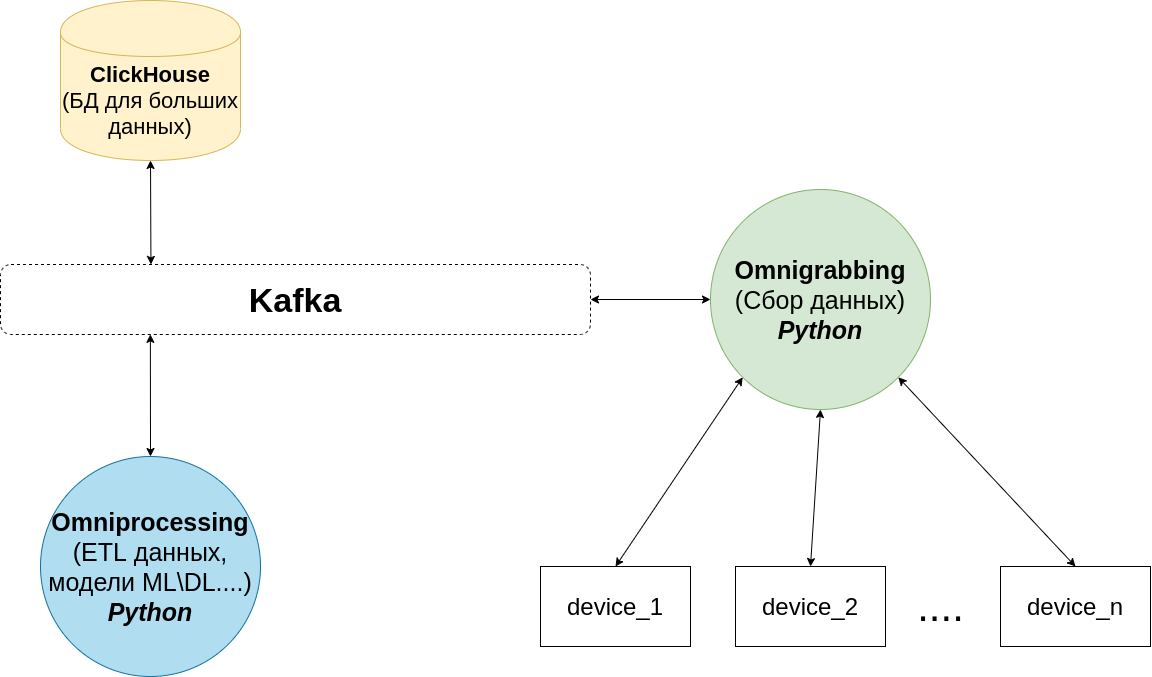
\includegraphics[width=15cm]{partsys2.png}}
    \caption{Часть системы, отвечающая за анализ и обработку данных}
    \label{partsys2}
\end{figure}

Микросервис omniprocessing (рисунок \ref{partsys2}) является местом, 
где располагаются различные модели для мониторинга и обработки данных,
например, модели машинного обучения.
Основные цели данного микросервиса -- извлечение, трансформация и загрузка.

В omniprocessing используется Python фреймфорк Faust, который позволяет отправлять
данные в очередь брокеру сообщений Kafka. Из Kafka данные попадают в базу данных ClickHouse.
Благодаря данному фреймворку можно быстро строить и встраивать пайплайны машинного обучения \cite{faust}. 
Разрабатываемое решение для станков Навигатор располагается именно
в микросервисе omniprocessing.


%-------------------------------------------------------------------------------

\subsection{LSTM нейронная сеть для прогнозирования временных рядов}

В последнее время использование нейронных сетей помогло улучшить
результаты решения большого количества задач в различных сферах человеческой деятельности.
Это обусловлено повышенными вычислительными мощностями современных компьютеров.
Именно повышение мощности позволило использовать теоретические изыскания
многих поколений ученых, занимающихся нейронными сетями, максимальным образом.

Область прогнозирования временных рядов не стала исключением
для улучшения результатов на основе использования нейронных сетей.
Наибольшего прорыва достигли LSTM или long-short term memory сети (долгосрочная краткосрочная память),
которые представляют собой разновидность архитектуры рекуррентной нейронной сети.

Рекуррентные нейронные сети, в отличие от однонаправленных многослойных перцептронов,
способны сохранять в памяти различные признаки, которые необходимы для поставленной задачи.
В случае временных рядов это могут быть долговременные зависимости, которые
могут влиять на прогноз.

\begin{figure}[H]
    \center{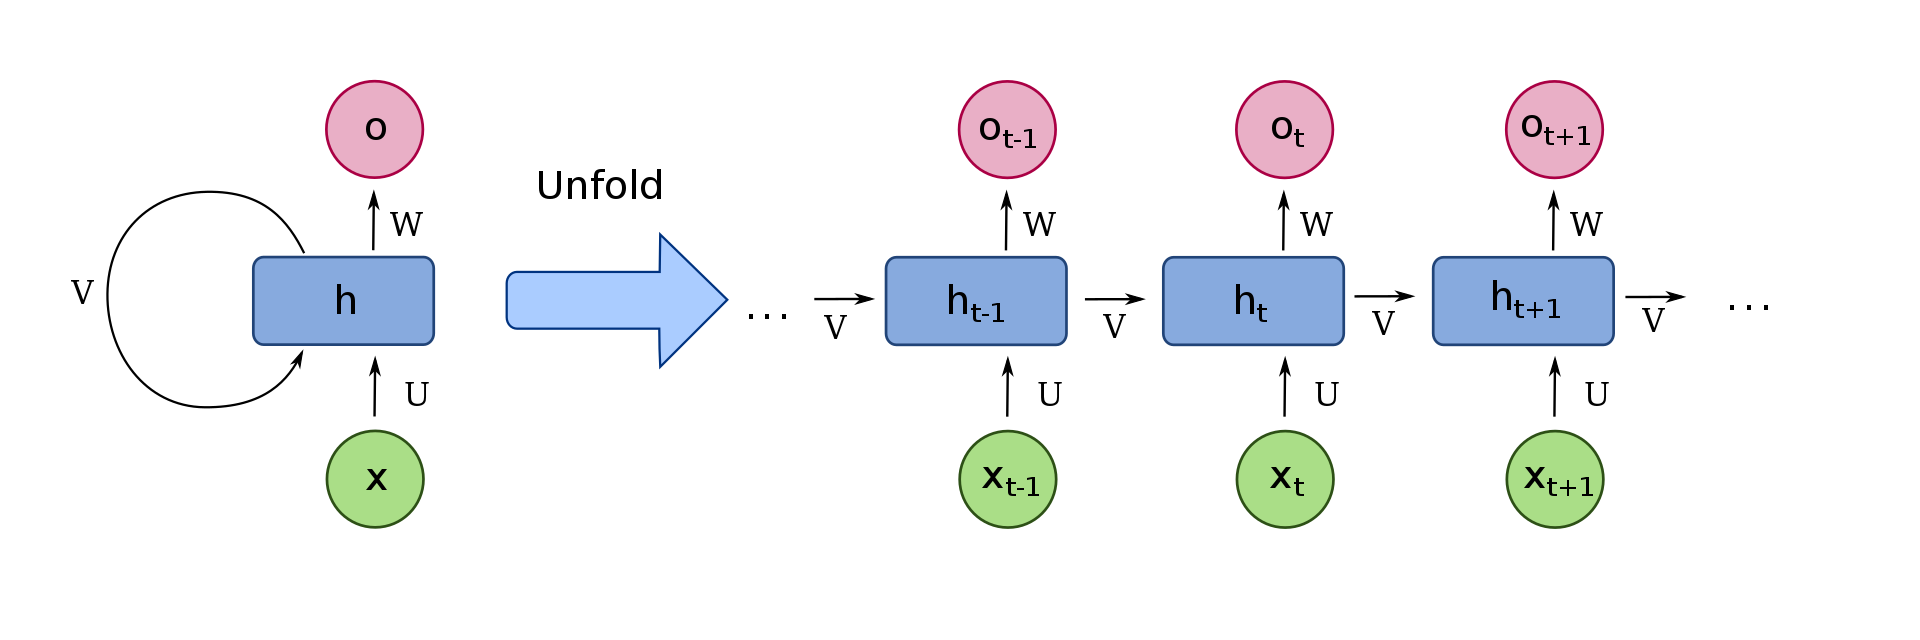
\includegraphics[width=15cm]{rnn.png}}
    \caption{Архитектура рекуррентной нейронной сети}
    \label{rnn}
\end{figure}

На рисунке \ref{rnn} отображена архитектура рекуррентной нейронной сети,
которая представляет собой направленную последовательность
узлов нейронной сети, каждый из которых
зависит и влияет на другие узлы на основе
перераспределения весов.

Пусть имеется матрица $X = \{\textbf{x}_1, ..., \textbf{x}_n \}$ входных данных
в нейронную сеть $h$, которая меняет свое состояние от $h_1$ до $h_n$,
с учетом последовательной обработки данных $X$ с различными временными шагами $t$,
а также на основе вычислений предыдущих шагов:

\begin{equation} \label{frnn}
    h_t = f(U\textbf{x}_t + V\textbf{x}_{t-1})
\end{equation}

Функция \ref{frnn} представляет собой функцию активации,
например, сигмоидальную функцию $\sigma$ или гиперболический тангенс $\tanh$,
либо совокупность функций активации,
которая зависит от конкретной архитектуры сети.
На каждом шаге $t$ нейронная сеть выдает результат $o_t$.
Матрицы $U$ и $V$ содержат входные и рекуррентные веса соответственно.

\begin{figure}[H]
    \center{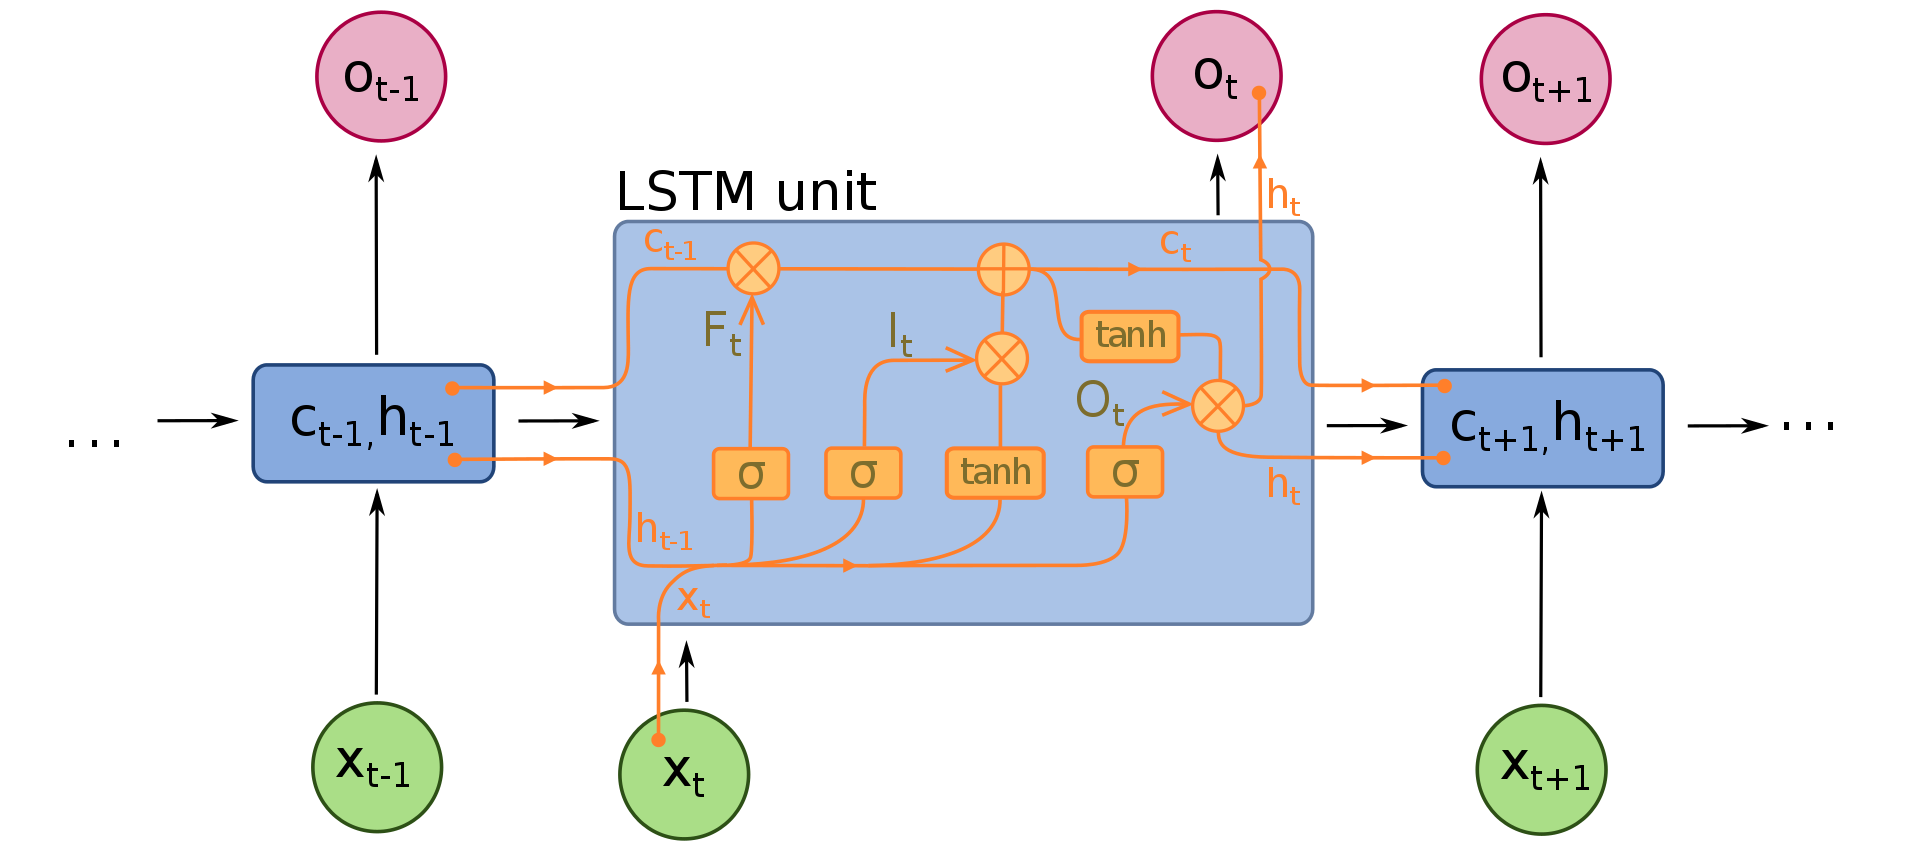
\includegraphics[width=15cm]{lstm.png}}
    \caption{Архитектура LSTM}
    \label{lstm}
\end{figure}

Рекуррентные нейронные сети
имеют различные архитектуры, каждая из которых имеет свои особенности,
достоинства и недостатки.
Самой эффективной для решения широкого спектра задач
является LSTM архитектура (рисунок \ref{lstm}).


\begin{equation} \label{lstmeq}
    \begin{gathered}
    F_t = \sigma(W_F x_t + U_F h_{t-1} + b_F) \\
    I_t = \sigma(W_I x_t + U_I h_{t-1} + b_I) \\
    \stackrel{\sim}{c}_t = \tanh(W_c x_t + U_c h_{t-1} + b_c) \\
    O_t = \sigma(W_O x_t + U_O h_{t-1} + b_O) \\
    c_t = F_t \circ c_{t-1} +  I_t \circ \stackrel{\sim}{c}_t
    h_t = o_t \circ \tanh(c_t)
    \end{gathered}
\end{equation}

Система уравнений \ref{lstmeq} описывает последовательность
вычислений нового скрытого состояния нейронной сети $h_t$.

\newpage

\begin{itemize}
    \item $F_t$ -- вектор активации забывающего узла;
    \item $I_t$ -- вектор активации входного обновляемого узла;
    \item $\stackrel{\sim}{c}_t$ -- вектор активации входящей клетки;
    \item $O_t$ -- вектор активации выходного узла;
    \item $c_t$ -- состояние клетки в момент $t$;
    \item $W$ и $U$ -- матрицы весов;
    \item $b$ -- вектор смещения.
\end{itemize}

%-------------------------------------------------------------------------------

\subsection{Оптимальное окно обучения}

Обычно, точность модели прогнозирования увеличивается
пропорционально количеству обучающих данных,
однако такой подход не всегда является подходящим.
При изменении поведения или статистики поступающих данных,
обученная модель может не отследить эти изменения,
что приведет к накоплению ошибок.
Такую проблему называют дрейфом концептов.
Для решения данной проблемы используется
движущееся окно для повторного обучения,
которое формируется по последним данным на основе заданного размера окна.

Выбор оптимального размера окна обучения моделей машинного обучения
является открытым вопросом.
Большой размер окна может иметь более точные результаты,
но это увеличивает сложность модели,
что делает ее непригодной для приложений реального времени,
тогда как небольшой размер окна
может привести к увеличению погрешности и, следовательно,
к снижению надежности системы, переобучению или недообучнению.

Авторы статьи \cite{optimal} предложили метод,
на основе которого определяется оптимальный размер обучающего окна.
Основная идея заключается в использовании 
спектрального анализа наименьших квадратов,
так же известного как метод Ломба-Скаргла.
Данный метод работает лучше на данных с пропусками, например,
такого похожего метода как быстрое преобразование Фурье.
Кроме этого, быстрое преобразование Фурье
требует равномерной распределенности данных,
которая не всегда возможна при анализе данных с датчиков устройств.

\begin{equation} \label{lomb}
    \begin{gathered}
    P_X(f) = \frac{1}{2\sigma^2} 
    \Bigg( 
        \frac{\big[
            \sum_{n=1}^N(x(t_n) - \overline{x})\cos(2\pi f(t_n-\tau))
        \big]^2}{\sum_{n=1}^N \cos^2(2\pi f(t_n-\tau))} \\
    + 
    \frac{\big[
            \sum_{n=1}^N(x(t_n) - \overline{x})\sin(2\pi f(t_n-\tau))
        \big]^2}{\sum_{n=1}^N \sin^2(2\pi f(t_n-\tau))}
    \Bigg)
\end{gathered}
\end{equation}



Функция \ref{lomb} является описанием метода Ломба-Скаргла.
Оптимальный размер обучающего окна определяется
на основе нахождения наибольшей периодической компоненты,
встречающейся в данных.
Другими словами, определяется
размер сезонности данных.
Однако, перед использованием данного метода данные необходимо 
протестировать на сезонность для того, чтобы убедиться корректности использования
данного метода.

\begin{equation} \label{tau}
    \tan(4\pi f \tau) = \frac{\sum_{n=1}^N \sin(4\pi f t_n)}{\sum_{n=1}^N \cos(4\pi f t_n)}
\end{equation}

Параметр $\tau$ определяется в уравнении \ref{tau}.

%-------------------------------------------------------------------------------

\subsection{Алгоритм k-Shape}

Для обнаружения аномалий или неисправностей в данных со станка необходимо использовать
основные принципы кластерного анализа, который представляет собой разбиение
данных на кластеры с целью выявления закономерностей.

Обычно задача кластеризации формулируется следующим образом.
Обозначим за $X = \{\textbf{x}_1, ..., \textbf{x}_n \}$ набор $n$ данных, где $\textbf{x}_i \in \mathbb{R}^m$.
При кластеризации данные $X$  необходимо разбить на $k$ непересекающихся кластеров $P = \{p_1, ..., p_k\}$ таким образом,
что сумма квадратов дистанций между экземпляром данных $x_i$ и центроидов $\textbf{c}_j$,
который представляет собой точку концентрации кластера $p_j$, минимальна:

\begin{equation} \label{clusters}
    P^* = \arg \min \sum_j^k \sum_{\textbf{x}_i \in p_j} dist(\textbf{x}_i, \textbf{c}_j)
\end{equation}

В Евклидовом пространстве подобная задача оптимизации является NP-полной.
Метод k-средних позволяет найти локальный оптимум посредством
случайного распределения $k$ центроидов среди данных.

В кластерном анализе существуют различные алгоритмы кластеризации,
каждый из которых имеет свою специфику и может зависеть
от структуры анализируемых данных.

В последние несколько десятилетий, кластеризация последовательностей временных рядов получила значительное внимание,
не только как мощный самостоятельный исследовательский метод,
но и также как один из множества шагов в исследовании и обработки данных.

Большинство методов анализа временных рядов, включая кластеризацию,
зависят от выбора меры расстояния. Ключевой вопрос при сравнении двух последовательностей 
временных рядов заключается в том, как обрабатывать различные искажения, 
которые характерны для временных последовательностей.

Из-за различных трудностей и потребностей в инвариантности относительно предметных областей,
большое внимание уделялось созданию новых мер расстояния, а не созданию новых алгоритмов кластеризации. 
Обычно считается, что выбор меры расстояния более важен, чем сам алгоритм кластеризации. 
Как следствие, кластеризация по временным рядам основывается главным образом на классических методах кластеризации: 
либо путем замены расстояния по умолчанию на более подходящее для временных рядов, 
либо путем преобразования временных рядов в «плоские» данные для того, чтобы существующие алгоритмы кластеризации 
могли быть использованы непосредственно.

Однако выбор метода кластеризации может повлиять
на точность, так как каждый метод выражает однородность и разделение кластеров по-разному, и эффективность, 
поскольку вычислительные затраты отличаются от одного метода к другому. Например, спектральная кластеризация 
или некоторые варианты иерархической кластеризации являются более подходящими для идентификации кластеров 
на основе плотности распределения (на основе областей с более высокой плотностью), 
чем методы разделения, такие как метод k-средних. С другой стороны, метод k-средних более эффективен,
чем иерархические или спектральные методы в общем случае. 

Современные подходы к кластеризации на основе формы данных,
в которых используются методы разбиения с мерами расстояния,
не зависящими от масштаба и сдвига, имеют два основных недостатка:
(i) эти подходы не могут масштабироваться до больших объемы данных, поскольку они зависят 
от вычислительно дорогостоящих методов или мер расстояния; 
(ii) эти подходы были разработаны для конкретных предметных областей или их эффективность была
показана только для ограниченного числа наборов данных. 
Более того, наиболее успешные методы кластеризации на основе форм обрабатывают 
фазовую инвариантность посредством локального нелинейного выравнивания координат 
последовательности, даже если глобальное выравнивание часто является адекватным. 

Описанные подходы никогда не подвергались
всесторонней оценке друг против друга, против других методов разделения или против различных подходов, 
таких как иерархические или спектральные методы.
Данный сравнительный анализ присутствует только частично в различных статьях.

В статье \cite{k-shape} авторы предложили новый алгоритм k-Shape для кластеризации временных рядов на основе форм данных, 
который эффективен и не зависит от конкретной предметной области.
k-Shape основан на масштабируемой процедуре итеративного уточнения, 
аналогичной той, которая используется алгоритмом k-средних, но с существенными отличиями. 
В частности, k-Shape использует и другую меру расстояния, и другой метод вычисления центроидов, чем метод k-средних.
Алгоритм k-Shape пытается сохранить формы последовательностей временных рядов при их сравнении. 
Для этого k-Shape требуется мера расстояния, которая инвариантна к масштабированию и сдвигу.
В отличие от других подходов кластеризации,
для k-Shape адаптируется статистическая мера кросс-корреляции.

Кросс-корреляция - это мера сходства сигналов с задержкой по времени,
которая широко используется для обработки сигналов и изображений.
Данная статистическая мера позволяет определить сходство
двух последовательностей $\textbf{x} = (x_1, ..., x_m)$
и $\textbf{y} = (y_1, ..., x_m)$ даже если они не выровнены
относительно друг друга (и даже если они имеют разную длину).
Инвариантность относительно сдвигов
достигается благодаря фиксированию
одной последовательности, например, $\textbf{y}$,
и последовательному скольжению $\textbf{x}$ через $\textbf{y}$,
при котором вычисляется скалярное произведение этих последовательностей.

В статье \cite{k-shape} авторы алгоритма k-Shape описали разбили этот алгоритм на три части:
k-shape, extract-shape и sdb. Опишем каждую часть.

На сначала вход алгоритму подается набор $z$-нормализованных временных рядов,
а также $k$ кластеров, количество которых определяется заранее,
что является отдельной задачей.

\begin{equation} \label{zscore}
    z_i = \frac{x_i-\mu}{\sigma}
\end{equation}

Уравнение \ref{zscore} описывает z-нормализацию, представляющую собой
отношение отклонения случайного элемента $x_i$
от математическое ожидания $\mu$ к стандартному отклонению $\sigma$.

\begin{figure}[H]
    \center{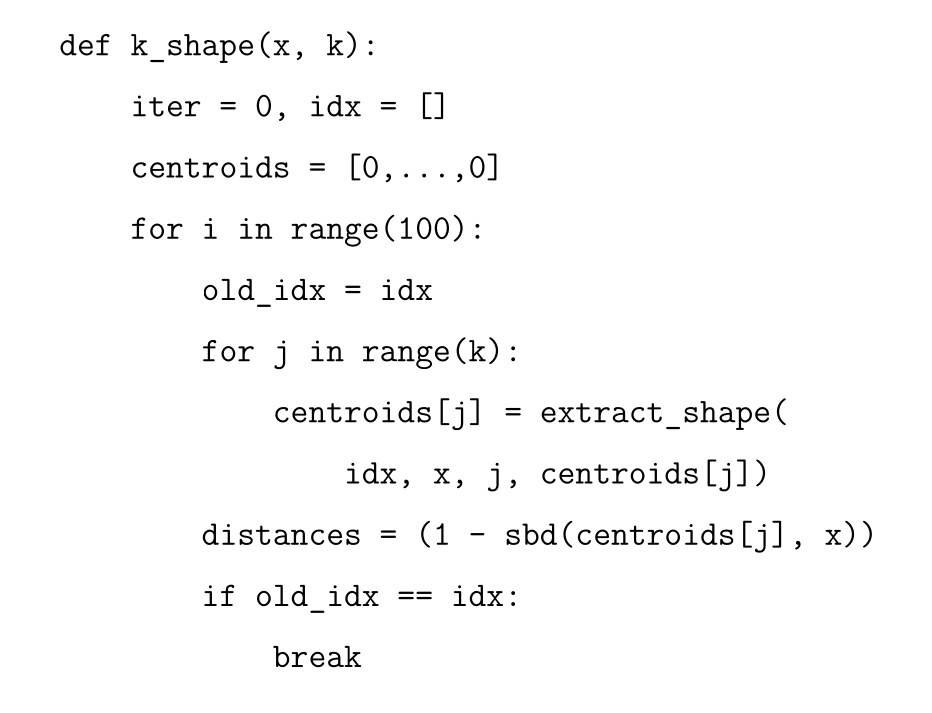
\includegraphics[width=13cm]{kshape.png}}
    \caption{Алгоритм k-Shape}
    \label{kshape}
\end{figure}

На рисунке \ref{kshape} отображен псевдокод алгоритма k-Shape.
На первом шаге инициализируются необходимые переменные:
счетчик итераций (iter), список для заполнения значений на основе кластеров (idx),
список заполненных нулями центроидов (centroids), длина которого зависит от количества кластеров $k$.
Далее происходят итерации, которые определяют центроиды и сами кластеры соответственно.
Авторы посчитали, что 100 итераций будет достаточно для нахождения локального оптимума.
Функция extract\_shape предназначена для вычисления нового центроида.
Функция sbd предназначена для вычисления так называемого shape-distance
нормализации коэффициентов кросс-корреляции.

\begin{figure}[H]
    \center{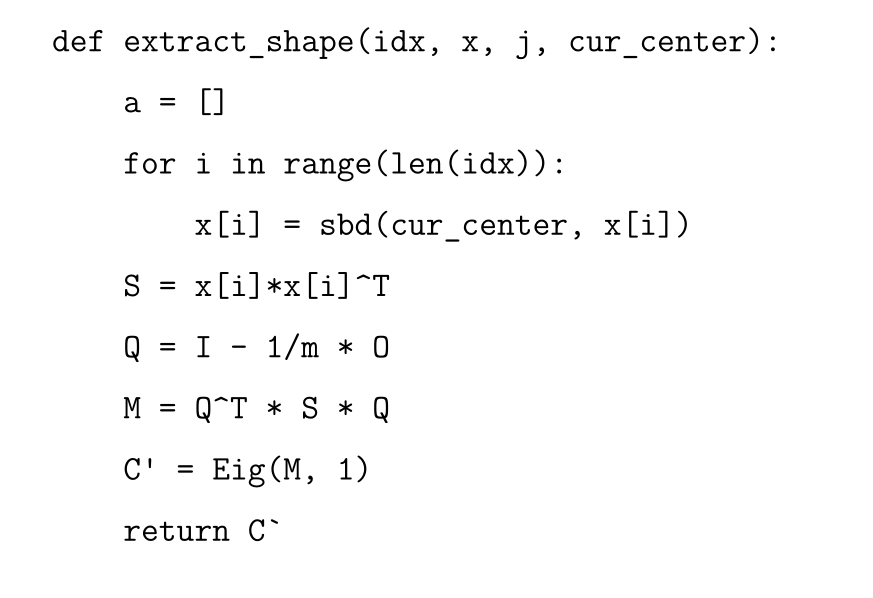
\includegraphics[width=13cm]{extract_shape.png}}
    \caption{Алгоритм вычисления нового центроида на основе расстояния SBD}
    \label{extract_shape}
\end{figure}

На рисунке \ref{extract_shape} отображен псевдокод вычисления нового центроида при помощи
максимизации квадратов SBD расстояний (уравнения \ref{sbd} и \ref{extraction}).
Матрицы $I$ и $O$ представляют собой единичную матрицу и матрицу, заполненную единицами.
В уравнении \ref{sbd} функция $CC(\textbf{x},\textbf{y})$ означает кросс-корреляцию,
$R_0$ -- функция автоматической кросс-корреляции.

\begin{equation} \label{sbd}
    SBD(\textbf{x}, \textbf{y}) = 1 - \max \Big( \frac{CC(\textbf{x},\textbf{y})}{\sqrt{R_0(\textbf{x}, \textbf{x})\cdot R_0(\textbf{y}, \textbf{y})}}\Big)
\end{equation}

\begin{equation} \label{extraction}
    \textbf{y}_k^*= \arg \max \sum_{\textbf{x}_i \in P_k}\Big(SBD(\textbf{x}_i, \textbf{y}_k)\Big)^2
\end{equation}

На основе свойств кросс-корреляции авторы алгоритма переписали исходное уравнение \ref{extraction}
в виде максимизации отношения Рэлея:

\begin{equation} \label{rel}
    \textbf{y}_k^* = \arg \max \frac{\textbf{y}_t^T \cdot M \cdot \textbf{y}_t}{\textbf{y}_t^T \cdot \textbf{y}_t}
\end{equation}

В уравнении \ref{rel} матрица $M$ является эрмитовой и имеет разложение Шура в виде $M = Q^T \cdot S \cdot Q$.
Вычисление матриц $Q$ и $S$ отображено в листинге 2.
Максимальное значение $\textbf{y}_k^*$ авторы нашли в качестве собственного вектора,
который соответствует максимальному собственному значению симметричной матрицы $M$.

\begin{figure}[H]
    \center{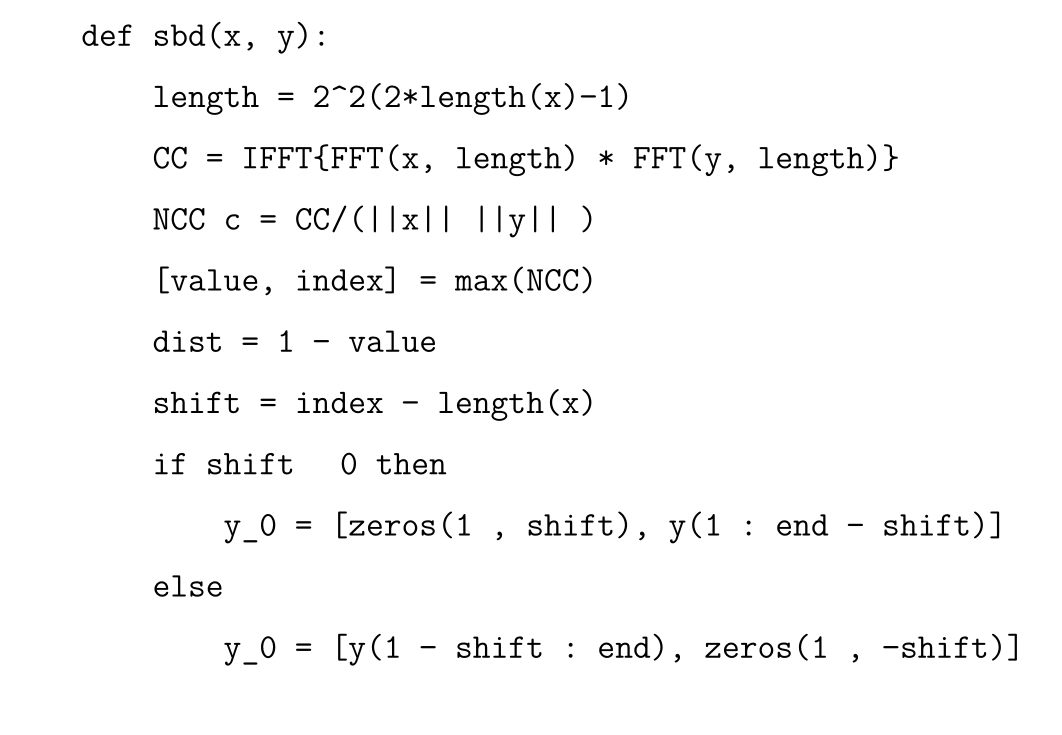
\includegraphics[width=13cm]{sbd.png}}
    \caption{Эффективное вычисление SBD расстояния}
    \label{sbdimg}
\end{figure}

На рисунке \ref{sbdimg} отображен алгоритм вычисления SBD расстояния
с использованием быстрого и обратного быстрого преобразования Фурье (FFT и IFFT).
Также, в данном листинге описаны последующие манипуляции с полученной
после работы с быстрым преобразованием Фурье кросс-корреляционной мерой.

%-------------------------------------------------------------------------------

\subsection{Градиентный бустинг}

Для выявления неисправностей необходима модель,
обученная на основе заданных критериев неисправностей и выявленных кластеров временных рядов.
Так как критерии и кластеры представляют собой выявленные признаки
на этапе анализа каждого временного ряда по отдельности,
необходимо использовать модель,
способную распознавать признаки
у всех временных рядов одновременного,
то есть, контексте данной работы,
определять неисправности на основе данных из различных датчиков
в виде многомерных временных рядов.

Для такой задачи лучше всего подходит подход на основе бустинга.
Бустинг -- это специальный алгоритм,
который основан на композиции других моделей машинного обучения.
Существуют различные модификации бустинга,
каждый из которых имеет свои особенности,
достоинства и недостатки.
Однако, в последнее время, наилучшие результаты
показывает алгоритм градиентного бустинга.

Градиентный бустинг -- разновидость бустинга,
в основе которого лежит
оптимизация дифференцируемой функции потерь
с использованием алгоритма градиентного спуска.
Опишем более формально данный алгоритм.

Пусть имеется набор данных $\{(\textbf{x}_i,y_i)\}_{i=1}^n$.
Необходимо найти аппроксимацию $\hat{F}$ функции $F(x)$,
которая минимизирует математическое ожидание
функции потерь $L(y, F(x))$ (уравнение \ref{lossgb}).

\begin{equation} \label{lossgb}
    \hat{F} = \arg \min \mathbb{E}[L(y, F(x))]
\end{equation}

Градиентный бустинг принимает $y$ и 
ищет аппроксимацию $\hat{F}$ на основе
взвешенных функций $h_i(x)$ из некоторого класса $H$,
называемых слабыми моделями обучения (уравнение \ref{gengb}).

\begin{equation} \label{gengb}
    \hat{F} = \sum_{i=1}^M \omega_i h_i(x) + const
\end{equation}

На первом шаге вычисляется функция $F_0$,
которая представляет себе первичную минимизацию функции потерь.

\begin{equation}
    F_0(x) = \arg \min \sum_{i=1}^n L(y_i, \omega)
\end{equation}

В итоге задается рекуррентное соотношение
метода градиентного спуска 
для функций потерь (уравнение \ref{gradgb}) и весов (уравнение \ref{wgb}).

\begin{equation} \label{gradgb}
    F_m(x) = F_{m-1}(x) - \omega_m \sum \nabla_{F_{m-1}} L(y_i, F_{m-1}(x_i))
\end{equation}

\begin{equation} \label{wgb}
    \omega_m = \arg \min \sum L(y_i, F_{m-1}(x_i) - \omega \nabla_{F_{m-1}} L(y_i, F_{m-1}(x_i))
\end{equation}

За счет оптимизации параметров множества слабых моделей,
градиентный бустинг способен выдавать результаты высокой точности.

%-------------------------------------------------------------------------------

\subsection{Инструменты для разработки моделей}

Для людей, занимающимися
анализом данных и машинным обучением,
существует множество инструментов для решения
различных их задач.
Инструменты могут представлять собой
как полноценную платформу (Matlab),
так и набор дополнительных программных пакетов (Python, R).

Разработка системы обнаружения
и прогнозирования неисправностей на станках лазерной резки
будет вестись с использованием языка программирования Python.
Данный язык выбран по двум причинам.
Во-первых, микросервис, в который будет внедрятся разрабатываемое решение,
как уже было описано, разработан на языке Python.
Во-вторых, для языка Python созданы гибкие и качественные
инструменты для манипуляции и анализа данных,
а также для инструменты для использования
последних достижений машинного обучения.

Основными инструментами для манипуляции с данными
являются библиотеки Numpy и Pandas.
Именно они используются для разработки.

Библиотека Numpy представляет собой
набор функций для операций над многомерными массивами.
Numpy хоть и используется для языка Python,
данная библиотека почти полностью написана на языке C,
поэтому она имеет высокие показатели производительности,
в отличие от стандартных инструментов,
которые предоставляет язык Python.

Pandas -- библиотека, позволяющая
быстро и гибко создавать комплексные датасеты,
а также предоставляющая эффективные методы
манипуляции с данными различного типа:
числовые, категориальные, временные, бинарные и т.д.

Для нужд описательной статистики,
а также для визуализации данных
используется библиотека Matplotlib.
Данный пакет содержит набор функций,
который позволяет строить двумерные
и трехмерные графики различной сложности.
Широкий функционал Matplotlib позволяет
наглядно анализировать данные,
а также отображать обработанные результаты.

Многие задачи машинного обучения
можно решить с использованием библиотеки машинного обучения Scikit-learn.
Данная библиотека предоставляет функционал для решения разнообразных
задач машинного обучения: регрессии, классификации, кластеризации, сокращения размерности и т.д.
Кроме этого, данная библиотека имеет возможности подготовки данных
для тренировки и тестирования моделей машинного обучения.
Данная библиотека будет использоваться именно для таких задач.


Библиотека Scikit-learn покрывает большое количество задач машинного обучения,
однако она не имеет подходящих инструментов для такой области как глубокое обучение.
Также очень часто из-за отсутствия оптимизации некоторых инструментов,
библиотека Scikit-learn может не подойти для использования в работающих системах,
поэтому ее в основном используют для прототипирования.
Поэтому были созданы библиотеки, в которых решены данные проблемы.
Нейронные сети, в том числе и используемые в работе LSTM,
можно использовать с помощью библиотек TensorFlow и Keras.

TensorFlow -- библиотека для задач машинного обучения и глубокого обучения в частности,
написанная на языке Python и C++,
с дополнительными возможностями использования технологии CUDA
-- технологии для параллельных вычислений на графических картах компании NVidia.
TensorFlow позволяет наглядно и быстро натренировать сложные модели машинного обучения,
а также быстро интегрировать и развернуть модели в рабочих средах.
Также данная библиотека может использоваться не только в языке Python,
но и в языках JavaScipt, C++ и Swift.

Keras представляет собой фреймворк для задач глубокого обучения,
включающий в себя инструменты для работы со сложными моделями глубокого обучения -- нейронным сетями различной архитектуры.
Keras создан на основе TensorFlow, что является преимуществом, так как фреймворк и библиотека способны работать согласованно.
Фреймворк Keras будет использоваться для тренировки нейронной сети LSTM.

\subsection{Выводы}

В данном разделе был проведен анализ системы компании Omnicube, в которую
будет интегрировано решение для прогнозирования и обнаружения ошибок станков Навигатор.

Для задач прогнозирования была выбрана рекуррентная нейронная сеть LSTM.
В разделе были описаны преимущества перед другими архитектурами нейронных сетей
для задач прогнозирования временных рядов.
Было дано подробное описание работы сети LSTM.
Также был описан принцип, по которому определяется оптимальное окно обучения.

Кроме этого, был проведен анализ алгоритмов кластеризации,
а также выбран и описан алгоритм k-Shape для кластеризации многомерных временных рядов.
Именно данный алгоритм поможет качественно определять особенности данных временных рядов станка Навигатор,
и на основе этих особенностей определять неисправности.

В конце раздела было дано краткое описание используемых для разработки инструментов,
а именно анализ библиотек и фреймворков для задач анализа данных и задач машинного обучения,
предназначенных для языка Python.



\clearpage